%!TEX program = lualatex
\documentclass[border=0mm,11pt]{standalone}
%\usepackage{color}
%\usepackage{tikz}
\usepackage[T1]{fontenc}
\usepackage[sc]{mathpazo}
\usepackage{tikz-feynman}
\tikzfeynmanset{compat=1.1.0}


\begin{document}

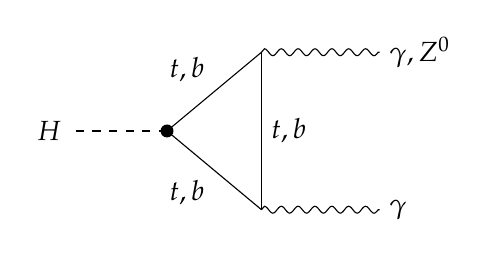
\begin{tikzpicture}[]
    \begin{feynman}
    \vertex (h) {$H$};
    \vertex [right=of h, xshift=-0.0cm, yshift=-0.0cm] (cent);
    \vertex [right=of cent, xshift=-0.3cm, yshift=1.0cm] (b);
    \vertex [right=of b, xshift=-0.0cm, yshift=-0.0cm] (a) {$\gamma, Z^{0}$};
    \vertex [right=of cent, xshift=-0.3cm, yshift=-1.0cm] (d);
    \vertex [right=of d, xshift=-0.0cm, yshift=-0.0cm] (c) {$\gamma$};

    \node [dot] at (cent) {};
    \diagram* {
    (a) -- [boson] (b) -- [edge label'=\({t,b}\)] (cent),
    (c) -- [boson] (d) -- [edge label=\({t,b}\)] (cent),
    (b) -- [edge label=\({t,b}\)] (d),
    (cent) -- [scalar] (h),
    };
    \end{feynman}
\end{tikzpicture}

\end{document}